
\section{Practical Framework}

\subsection{Sprint 3}

\subsubsection{Introduction}
During this sprint the team focused on the implementation of the input handler and input handler for bridge, as well as input management and sound management. The UMLs of each were assigned and based on these, implementation tasks were assigned based on the UMLs.

\subsubsection{POCs}

No proofs of concept (POCs) were conducted in this sprint.

\subsubsection{Technical Justification}
In Sprint 3 the decision was made to design the UMLs and implement them. The decision was made based on the following:

\begin{itemize}
    \item  Being able to handle keyboard and mouse events
    \item  Hear the sounds of the game through the console.
    \item  Communicate game with console.
    \item  Handle the updates of the information beetwen game and console.
\end{itemize}

\newpage

\subsubsection{Product Backlog}

\documentclass{article}
\setcounter{secnumdepth}{3}

\usepackage{amsmath,amssymb}
\usepackage{lmodern}
\usepackage{iftex}
\usepackage[letterpaper, margin=1in, top=0.5in, bottom=1in]{geometry}
\usepackage{listings}
\usepackage{color}
\usepackage{titling}
\usepackage{graphicx}
\usepackage{hyperref}
\usepackage{parskip}

\begin{document}

\maketitle

\hypertarget{burndownchart-s3}{
\section{Burn Down Chart}\label{Burn Down Chart S3}}
\href{https://tree.taiga.io/project/joseluis-teran-coffeetime/taskboard/sprint-3-8974}{Link: Sprint 3 Board on Taiga}.

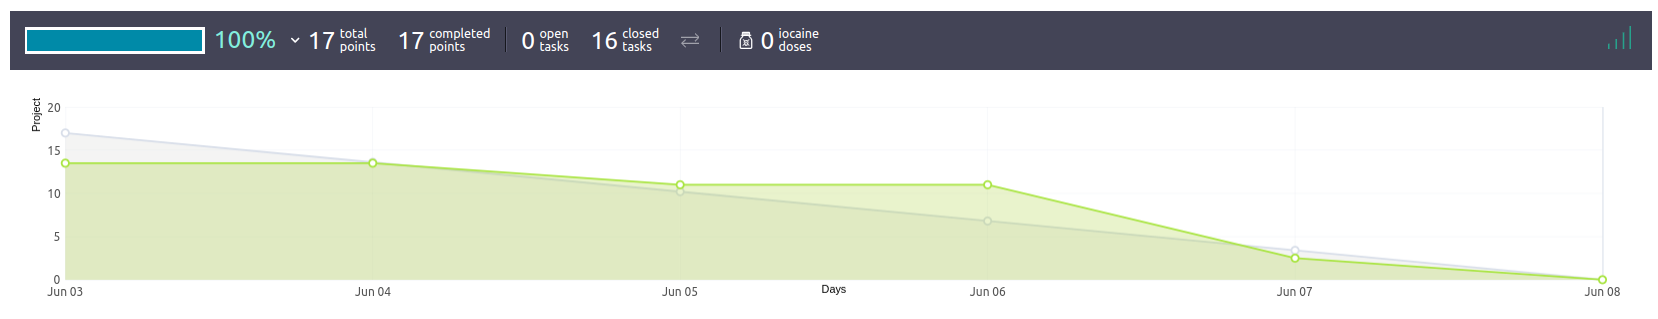
\includegraphics[width=\textwidth]{./assets/burndown-s3.png}

\hypertarget{startstopcontinueactionitems-s3}{
\section{Start-Stop-Continue-Action Items}\label{Start-Stop-Continue-Action Items S2}}
\href{https://miro.com/app/board/uXjVKDO7l8M=/?moveToWidget=3458764590247889881&cot=14}{Link: Start-Stop-Continue-Action Items Sprint 3 on Miro}.

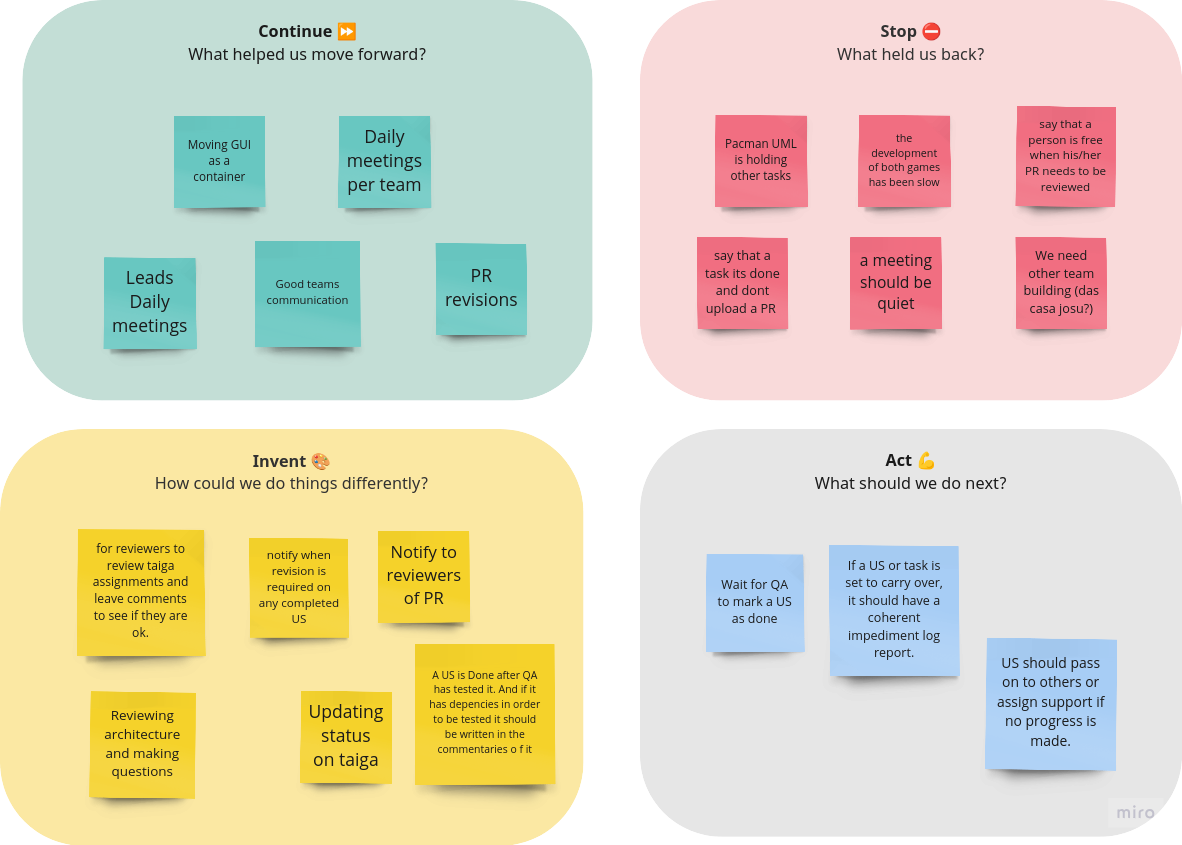
\includegraphics[width=\textwidth]{./assets/retrospective-s3.png}

\end{document}


\paragraph{Impediments}
For the impediments we registered on the following link:

\href{https://docs.google.com/spreadsheets/d/1hnMwOOVtyGWhViuAGwBsDpP79jTbHlJ09a_0gc9b4CM/edit?gid=1617748097#gid=1617748097}{impediments}

\paragraph{Conclusions}

For sprint 3 our goal was to implement in the project the different parts of the architecture to communicate with each other in the future, but this goal could not be fully achieved as some parts could not be implemented within the sprint duration.

\subsubsection{action items}

\begin{itemize}
    \item US should pass on to others or assign support if no progress is made.
    \item If a US or task is set to carry over, it should have a coherent impediment log report.
\end{itemize}

\subsubsection{Epics}

For Sprint 3 we have the following epics:

\begin{itemize}
    \item Input Management
    \item Sound management
    \item Input handler for the bridge
    \item Update Handler
    \item UML Pacman Game
    \item Render handler implementation 
\end{itemize}